\iffalse
\let\negmedspace\undefined
\let\negthickspace\undefined
\documentclass[journal,12pt,twocolumn]{IEEEtran}
\usepackage{cite}
\usepackage{amsmath,amssymb,amsfonts,amsthm}
\usepackage{algorithmic}
\usepackage{graphicx}
\usepackage{textcomp}
\usepackage{xcolor}
\usepackage{txfonts}
\usepackage{listings}
\usepackage{enumitem}
\usepackage{mathtools}
\usepackage{gensymb}
\usepackage{comment}
\usepackage[breaklinks=true]{hyperref}
\usepackage{tkz-euclide} 
\usepackage{listings}
\usepackage{gvv} 
\usepackage{caption}
\def\inputGnumericTable{}                                 
%\usepackage[latin1]{inputenc}                                
\usepackage{color}                                            
\usepackage{array}                                            
\usepackage{longtable}                                       
\usepackage{calc}                                             
\usepackage{multirow}                                         
\usepackage{hhline}                                           
\usepackage{ifthen}                                           
\usepackage{lscape}

\newtheorem{theorem}{Theorem}[section]
\newtheorem{problem}{Problem}
\newtheorem{proposition}{Proposition}[section]
\newtheorem{lemma}{Lemma}[section]
\newtheorem{corollary}[theorem]{Corollary}
\newtheorem{example}{Example}[section]
\newtheorem{definition}[problem]{Definition}
\newcommand{\BEQA}{\begin{eqnarray}}
\newcommand{\EEQA}{\end{eqnarray}}
\newcommand{\define}{\stackrel{\triangle}{=}}
\theoremstyle{remark}
\newtheorem{rem}{Remark}

\begin{document}

\bibliographystyle{IEEEtran}
\vspace{3cm}

\title{NCERT 12.10 5Q}
\author{EE23BTECH11013 - Avyaaz$^{*}$% <-this % stops a space 
}
\maketitle
\newpage
\bigskip

\renewcommand{\thefigure}{\arabic{figure}}
\renewcommand{\thetable}{\arabic{table}}

\large\textbf{\textsl{Question:}}
In Young’s double-slit experiment using monochromatic light of wavelength $\lambda$, the intensity of light at a point on the screen where path difference is $\lambda$, is $K$ units. What is the intensity of light at a
point where path difference is $\lambda$/3?\\
\large\textbf{\textsl{Solution:}}
\fi
\begin{table}[htbp]
\setlength{\extrarowheight}{8pt}
\centering
\begin{tabular}{|c|c|c|}
\hline 
   \textbf{Parameter}  &\textbf{Description} &\textbf{Value} \\
\hline
$y_i\brak{t}$ & Equation of light from $ S_{i^\text{th}}$ &  $A\sin(\omega t  - kx_i)$ \\
\hline
$k $ & Wave number &$ \dfrac{2\pi}{\lambda}$  \\[5pt]
\hline
$I $&  Intensity of wave  &$ \propto A^2$  \\
\hline
\multirow{3}{*}{$\Delta x = x_1 - x_2$} & \multirow{3}{*}{Path difference} & $\lambda$ \\
\cline {3-3}
& & $\dfrac{\lambda}{3}$ \\
\hline
$K$ & Intensity of light at $\Delta x = \lambda$ & \\
\hline
$A$&Amplitude of wave from source&\\
\hline
$r$ & constant & $r \geq 0$ \\
% $I_1$&Intensity of light at individual slits&$\dfrac{K}{4}$ \\ 
% \hline
% $I_r$&Net Intensity of light at $\Delta x =\dfrac{\lambda}{3}$ &$\dfrac{K}{4}$ \\
\hline
\end{tabular}

\caption{Parameters}
\label{tab:parameters}
\end{table}

From \tabref{tab:parameters}:
\begin{align}
%%y\brak{t} &= y_1\brak{t} + y_2\brak{t}  \\
y\brak{t} &= A\sin({2\pi f t - kx_1})  + A\sin({ 2\pi f t - kx_2}) \\
y\brak{t} &=  2A\cos\left(\dfrac{k\Delta x}{2}\right)\sin\left(2\pi f t - \dfrac{k(x_1+x_2)}{2} \right) \label{eq:superposition}
\end{align}
From \tabref{tab:parameters} and equation \eqref{eq:superposition}: 
\begin{align}
\therefore I \propto 4A^2\cos^2\left(\dfrac{k\Delta x}{2}\right)  \label{eq:intensity}
\end{align}
From \tabref{tab:parameters} and equation \eqref{eq:intensity}: 
\begin{align}
 \dfrac{K}{I_r} = \dfrac{4A^2\cos^2\left(\dfrac{2\pi}{2}\right)}{4A^2\cos^2\left(\dfrac{\pi}{3}\right)}
 \implies I_r = \dfrac{K}{4}
 \end{align}
 Hence, the Intensity of light at a point where path difference is $\dfrac{\lambda}{3}$ is $\dfrac{K}{4}$ units.

\begin{table}[htbp]
\centering
\begin{tabular}{|c|c|c|}
\hline 
   \textbf{Parameter}  &\textbf{Description} &\textbf{Value} \\
\hline
&&\\
$I_r$&Net Intensity of light at $\Delta x =\dfrac{\lambda}{3}$ &$\dfrac{K}{4}$ \\&&\\
\hline
\end{tabular}

\caption{}
\label{tab:intensity}
\end{table}
Assuming $\Delta x= r\lambda$, 

From equation \eqref{eq:intensity}:
\begin{figure}[htbp]
    \centering
    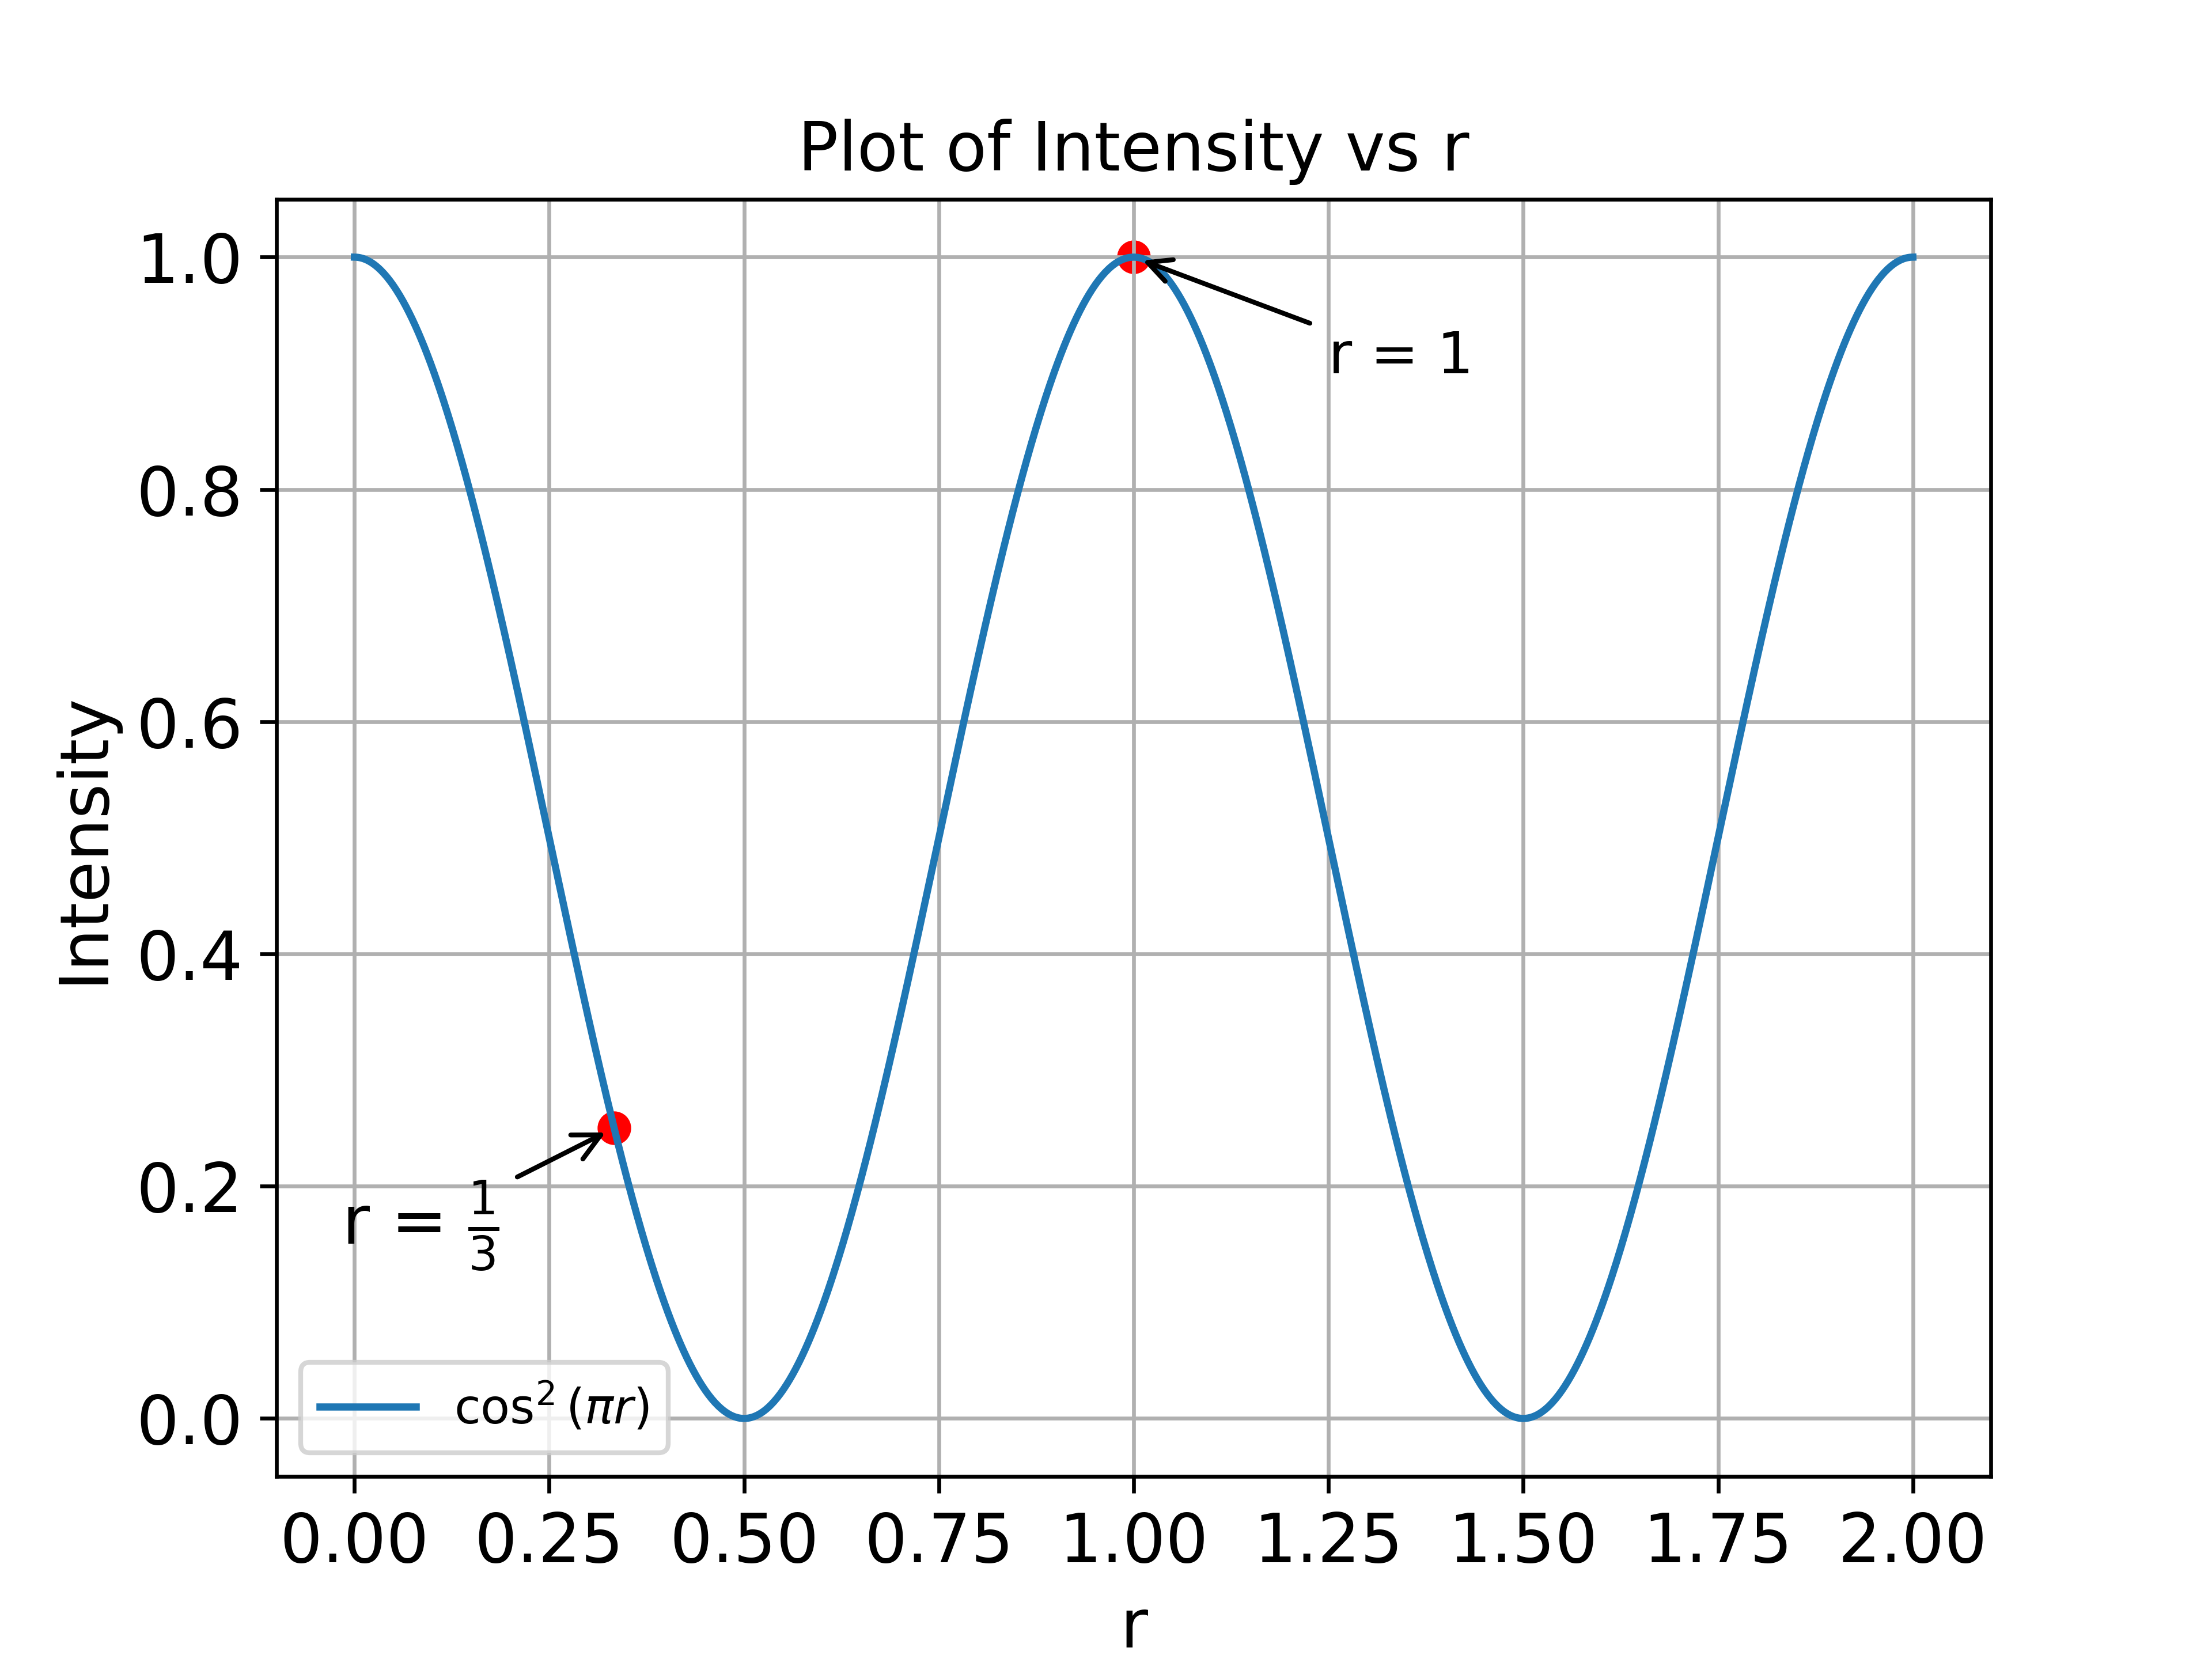
\includegraphics[width = \columnwidth]{ncert-physics/12/10/5/figs/intensity_plot.png}
  \caption{}
    \label{fig:graph1}
\end{figure}
\bibliographystyle{IEEEtran}
%\end{document}
